\chapter{Architecture}
\label{chapter:architecture}

Alcaudon's architecture will be described in this chapter following a top-down
approach. Firstly, a general description of the different components of the system
will be explained. Finally, each of the components will be described more thoroughly.

\subsection{General description}

Alcaudon's platform is composed by 3 main units.

\begin{itemize}
\item \textbf{Alcaudon library}: This is the main interface between users
  and the system. In order to use Alcaudon it is necessary to have access to a
  cluster with a coordinator and computing nodes. This interface is provided as
  a library containing the tools to build dataflows, the interfaces to implement
  user defined stream computations and the tools to connect with a particular
  cluster. Since the computations are potentially infinite, the operations
  performed against the cluster are asynchronous, returning an id associated
  with the created operation.
\item \textbf{Coordinator node}: This is the main component of the system. It
  coordinates the life cycle of the different components of the cluster such as
  the computing nodes. It is also responsible of performing the scheduling of
  the user defined dataflows given the resources provided by the computing
  nodes. Finally, it is the interface between the cluster and the users, where
  they deploy their dataflow topologies.

\item \textbf{Computing nodes}: These nodes are in charge of executing the
  actual computations provided by Alcaudon's users. These nodes take care of
  storing intermediate results published to streams. They register dynamically
  to the cluster contacting the coordinator node. A deployment can be composed
  from one computing node up to thousands, as needed. Each of these nodes
  provides certain resources to the system, known as \textit{computation slots}.
  The number of slots is configurable, but they correlate with the number of
  available CPU's in the underlying hardware.
\end{itemize}

A high level overview of the system can be seen in
figure~\ref{fig:architecture}. The majority of the parts of the system have been
modeled as Actors. As it was stated previously it is a very good fit for this
kind of applications. Where possible, object oriented design patterns\cite{gof}
such as \textbf{builder} or \textbf{factory} have been used. However, functional
programming constructs such as monads\cite{monads}, type
classes\cite{typeclasses} or Algebraic Data Types have been used more widely.

Once the different parts of the system have been presented, they will be
inspected in detail.

\begin{figure}[!h]
  \centering
  \includegraphics[width=0.9\textwidth]{architecture.pdf}
  \caption{Alcaudon architecture schema}
  \label{fig:architecture}
\end{figure}

\newpage
\subsection{Alcaudon library}

In the first place, the user facing interface will be presented in detail. In order
to create a streaming data processing pipeline, or dataflow topology as it has
been defined during all this document, users should provide their business
logic. To achieve this goal, Alcaudon provides certain interfaces so users
just need to care about their code. These interfaces are available as a library
that can be found at at Sonatype OSSRH \footnote{http://central.sonatype.org/pages/ossrh-guide.html}.

\begin{figure}[!h]
  \begin{center}
  \includegraphics[width=0.6\textwidth]{client.pdf}
  \caption{Alcaudon library}
  \label{fig:library}
  \end{center}
\end{figure}

This library is composed of three modules as it is shown in figure~\ref{fig:library}:

\begin{itemize}
\item Computation API's: Interface that users should implement in order to
  create computations.
\item Dataflow builder: This component is used to build dataflow topologies and
  later on submit the to the cluster coordinator.
\item Cluster client: Communication layer between clients and Alcaudon clusters.
  It handles all the operations needed to submit custom code to the cluster as well
  as the stream processing pipeline definition.
\end{itemize}

\subsubsection{Computation API's}

\begin{figure}[!h]
  \begin{center}
  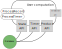
\includegraphics[width=0.5\textwidth]{libraryApi.pdf}
  \caption{Alcaudon computation API's}
  \label{fig:apis}
  \end{center}
\end{figure}

As explained before, in order to create custom computations to process unbounded
data-sets in Alcaudon, it is necessary to implement an interface. The interface
is listed in~\ref{code:computation}. This interface gives access to the
abstractions provided by the system as represented in figure~\ref{fig:apis}. As
it can be observed, there are two methods to be implemented;
\lstinline[columns=fixed]{def processRecord(record: Record): Unit} and \lstinline[columns=fixed]{def processTimer(timer: Timer): Unit}.

\begin{lstlisting}[language=scala, frame=trBL, label=code:computation, float=ht, caption = {Computation API's}]
trait Computation
    extends ProduceAPI
    with TimerAPI
    with StateAPI
    with SerializationAPI
    with RuntimeContext {
  ...
  def processRecord(record: Record): Unit
  def processTimer(timer: Timer): Unit
  ...
}
\end{lstlisting}

These methods represent the main entry point into user code, hooked in reaction to
record receipt and timers expiration. These constitute the application logic.
Within the execution of these methods, Alcaudon provides different functions to
work with persistent state, publish new records to streams, set timers or
serialize arbitrary data types. Those auxiliary API's are listed
in~\ref{code:auxiliaryComputations}. In Alcaudon, each computation can subscribe to
multiple sources represented as streams. Data travels in its simplest form,
as an array of bytes.

\begin{figure}[!h]
  \begin{center}
    
\includegraphics[width=0.5\textwidth]{keypartitioning.pdf}
    \caption{Alcaudon record key assignment}
    \label{fig:keypartitioning}
  \end{center}
\end{figure}

However, for each stream subscription users should provide
a key extraction function, this process can be shown in figure
~\ref{fig:keypartitioning}. Having a key per record allows the implementation of
parallelization strategies such as key partitioning. Therefor, every record
emitted by one of the subscribed sources, an instance of the class
\lstinline[columns=fixed]{Record} listed in ~\ref{code:records} will be
injected with the call to \lstinline[columns=fixed]{processRecord}.

\begin{lstlisting}[language=scala, frame=trBL, label=code:records, float=ht, caption = {Record classes}]
case class RawRecord(value: Array[Byte], timestamp: Long) {
  val id = UUID.randomUUID().toString
}
case class Record(key: String, rawRecord: RawRecord) {
  val value = rawRecord.value
  val timestamp = rawRecord.timestamp
  val id = UUID.randomUUID().toString
}
\end{lstlisting}

Timers are the other possible trigger for user defined code execution. In
Alcaudon there are three types of timers:

\begin{itemize}
\item \textit{Fixed timers}: This kind of timers are triggered once at a
  specific wall time.
\item \textit{Recurrent fixed timers}: This timer is just like the previous
  timers, however it is executed recurrently. I.E., every five minutes.
\item \textit{Watermark timers}: This timer try to estimate the point where all
  the events up to certain window have been consumed by the system and execute
  then. The mechanism and algorithm used to implement them will be explained
  later.
\end{itemize}

When a timer is executed it has as a parameter an instance of the class Timer
listed in ~\ref{code:timers}. This constructs are key to the domain of unbounded
data-sets due to its very nature. A mean to emit partial results is needed, so
this is the mechanism provided by Alcaudon to emit results.

\begin{lstlisting}[language=scala, frame=trBL, label=code:timers, float=ht, caption = {Timer class}]
  case class Timer(tag: String, timestamp: Long)
\end{lstlisting}

\subsubsection{Dataflow builder}

Once the computations are implemented, users need a way to build the dataflow topologies.
To achieve this goal, the system provides a dataflow builder. It is based on a very well
known design pattern, the builder pattern. Using this class, users are able to define
the dependencies among the main entities in the system. These main entities are:

\begin{itemize}
  \item \textit{Sources}: 
  \item \textit{Computations}:
  \item \textit{Streams}:
  \item \textit{Sinks}:
\end{itemize}


MOVE 
\begin{lstlisting}[language=scala, frame=trBL, label=code:auxiliaryComputations, float=ht, caption = {Computation API's}]
trait ProduceAPI { environment: RuntimeContext =>
  protected def produceRecord(record: RawRecord, stream: String): Unit =
}

trait TimerAPI { environment: RuntimeContext =>
  protected def setTimer(timer: Timer): Unit
}

trait StateAPI { environment: RuntimeContext =>
  protected def set(key: String, value: Array[Byte]): Unit
  protected def get(key: String): Array[Byte]
}

trait SerializationAPI {
  def serialize[T](data: T)(implicit ti: TypeInfo[T]): Array[Byte]
  def deserialize[T](binary: Array[Byte])(implicit ti: TypeInfo[T]): T
}
\end{lstlisting}
